% !TEX root = ../main.tex
\chapter{Convolutional Neural Networks (CNN)}

\section{What Is a Convolutional Neural Network?}

A Convolutional Neural Network (CNN) is a type of neural network designed to process images by using small kernels (or filters) that slide across the image. Instead of learning separate weights for every input-output connection, the CNN learns only the kernel's weights and reuses them at every position in the image.

As the kernel moves across the image, it computes an output value at each location. Collecting all these outputs produces a \textbf{feature map}, which shows how strongly the learned pattern (such as an edge or corner) appears at every location in the image.

\section{The Problem with Traditional Fully Connected Neural Networks}

When images are processed using a traditional fully connected neural network (MLP), the image must first be flattened into a one-dimensional vector. This creates two major problems: a very large number of parameters and the loss of the image's spatial structure.

For example, connecting a $28 \times 28$ image (784 pixels) to a layer of 128 neurons requires:

\[
784 \times 128 = 100,352 \text{ weights}
\]

Moreover, the network treats each pixel independently, without explicitly considering the spatial relationships between neighboring pixels.

\section{The CNN Solution}

A Convolutional Neural Network (CNN) addresses these limitations through \textbf{local connectivity} and \textbf{parameter sharing}. Rather than connecting every input pixel to every neuron, it uses a small number of learnable parameters to extract local patterns from the image.

For example, a $3 \times 3$ kernel contains only 9 weights (ignoring the bias), compared with the 100,352 weights required by the MLP example above. These parameters are reused across different image locations, significantly reducing the number of learnable parameters.

\begin{itemize}
    \item \textbf{MLP:} 784 inputs $\rightarrow$ 100,352 weights, with each input connected to all 128 neurons.
    \item \textbf{CNN:} One $3 \times 3$ kernel $\rightarrow$ 9 weights (ignoring the bias), reused across the image to detect the same pattern at different locations.
\end{itemize}


\clearpage
\begin{figure}[htbp]
    \centering
    \includegraphics[width=0.92\textwidth]{2-saddle point - CNN/photo_5_2026-07-28_02-59-38.jpg}
    \caption{CNN Structure Overview showing feature extraction layers and MLP classification head.}
    \label{fig:cnn_structure}
\end{figure}

\clearpage
\section{Convolution Operation}

An RGB image is composed of three channels: red, green, blue. Each channel containing intensity values of one color. During Convolution, a kernel passes across all three channels simultaneously. The filter has the same depth as the input.

\begin{center}
\begin{minipage}{0.45\textwidth}
\centering
\textbf{Input Image ($5 \times 5$)} \\[0.4em]
\begin{tabular}{|c|c|c|c|c|}
\hline
12 & 255 & 128 & 12 & 13 \\ \hline
1 & 11 & 12 & 14 & 15 \\ \hline
115 & 30 & 40 & 16 & 17 \\ \hline
18 & 19 & 20 & 21 & 22 \\ \hline
23 & 24 & 25 & 26 & 27 \\ \hline
\end{tabular}
\end{minipage}
\quad $\mathbf{\times}$ \quad
\begin{minipage}{0.35\textwidth}
\centering
\textbf{Kernel ($3 \times 3$)} \\[0.4em]
\begin{tabular}{|c|c|c|}
\hline
-1 & -1 & -1 \\ \hline
0 & 0 & 0 \\ \hline
1 & 1 & 1 \\ \hline
\end{tabular}
\end{minipage}
\end{center}

Computes a weighted sum of local pixel values:
\begin{equation}
32 \times 32 \times 3 \xrightarrow{\text{Conv } 3 \times 3 \times 3} 30 \times 30 \times 1
\end{equation}

Repeating this process across the entire image creates a feature map that highlights specific patterns.

\section{Kernel (Filter)}

A kernel is a small matrix of learnable weights responsible for extracting features from an image, such as edges, corners, and textures. It slides across the image, performing element-wise multiplication with local pixel values and summing the results to produce a feature map. Its weights are initially assigned random values and gradually updated during training through backpropagation and gradient descent to learn useful visual features.

\section{Output Dimension \& Zero Padding}

The output size after a Convolution depends on four things:
\begin{itemize}
    \item Input size ($N$)
    \item Kernel size ($K$)
    \item Stride ($S$)
    \item Padding ($P$)
\end{itemize}

\begin{equation}
\text{Output Size} = \left\lfloor \frac{N - K + 2P}{S} \right\rfloor + 1
\end{equation}

\begin{equation}
\text{Example: } \left( \frac{32 - 3 + 2(0)}{1} \right) + 1 = 30 \quad (30 \times 30)
\end{equation}

\paragraph{Convolution: Zero Padding}
\begin{itemize}
    \item \textbf{Problem:} The output is smaller than the input. If the input is $28 \times 28$ and the filter is $3 \times 3$, you can have at most 13 convolutional layers (the output of the 13th layer is $2 \times 2$).
    \item \textbf{Solution (Zero Padding):} Adds a border of zeros around the input image before applying the convolution. This preserves more edge information and can keep the output size the same as the input (for example, using a $3 \times 3$ kernel with padding 1 and stride 1).
\end{itemize}

\section{Stride}

\begin{itemize}
    \item \textbf{Stride = 1:} The kernel moves 1 step each time.
    \item \textbf{Stride = 2:} The kernel moves 2 steps each time.
\end{itemize}

Using a Stride of 1 makes the kernel move one pixel at a time, producing large feature maps and increasing computation and memory usage. A large Stride moves the kernel more than one pixel at once, reducing the size of the output feature map. This decreases computation and memory requirements while preserving the most important features.

\begin{figure}[htbp]
\centering
\begin{tikzpicture}[scale=0.75]
  % Stride = 1 Illustration
  \begin{scope}[shift={(0,0)}]
    \node[anchor=west, font=\sffamily\bfseries\small, color=primaryblue] at (-0.5, 3.6) {Stride = 1 (1 step per shift)};
    \draw[step=0.8cm, warmgray!50, thin] (0,0) grid (4,3.2);
    % Step 1 box
    \draw[line width=1.4pt, secondaryblue, fill=secondaryblue!15] (0, 0.8) rectangle (1.6, 2.4);
    \node[font=\sffamily\tiny, secondaryblue] at (0.8, 1.6) {Step 1};
    % Step 2 box (shifted by 1)
    \draw[line width=1.2pt, accentred, dashed] (0.8, 0.8) rectangle (2.4, 2.4);
    \node[font=\sffamily\tiny, accentred] at (1.6, 1.0) {Step 2};
    \draw[-{Latex}, secondaryblue, thick] (0.8, 2.6) -- (1.6, 2.6) node[midway, above, font=\tiny] {+1 cell};
  \end{scope}

  % Stride = 2 Illustration
  \begin{scope}[shift={(7.5,0)}]
    \node[anchor=west, font=\sffamily\bfseries\small, color=primaryblue] at (-0.5, 3.6) {Stride = 2 (2 steps per shift)};
    \draw[step=0.8cm, warmgray!50, thin] (0,0) grid (4.8,3.2);
    % Step 1 box
    \draw[line width=1.4pt, secondaryblue, fill=secondaryblue!15] (0, 0.8) rectangle (1.6, 2.4);
    \node[font=\sffamily\tiny, secondaryblue] at (0.8, 1.6) {Step 1};
    % Step 2 box (shifted by 2)
    \draw[line width=1.2pt, accentred, dashed] (1.6, 0.8) rectangle (3.2, 2.4);
    \node[font=\sffamily\tiny, accentred] at (2.4, 1.6) {Step 2};
    \draw[-{Latex}, accentred, thick] (0.8, 2.6) -- (2.4, 2.6) node[midway, above, font=\tiny] {+2 cells};
  \end{scope}
\end{tikzpicture}
\caption{Visual illustration of Stride operation mechanism across feature grids.}
\label{fig:stride_diagram}
\end{figure}

\section{Pooling}

Pooling is a downsampling operation that reduces the spatial dimension (height and width) of a feature map while retaining its most important information. It helps reduce computation, memory usage, and the risk of overfitting.
\begin{figure}[H]
\centering
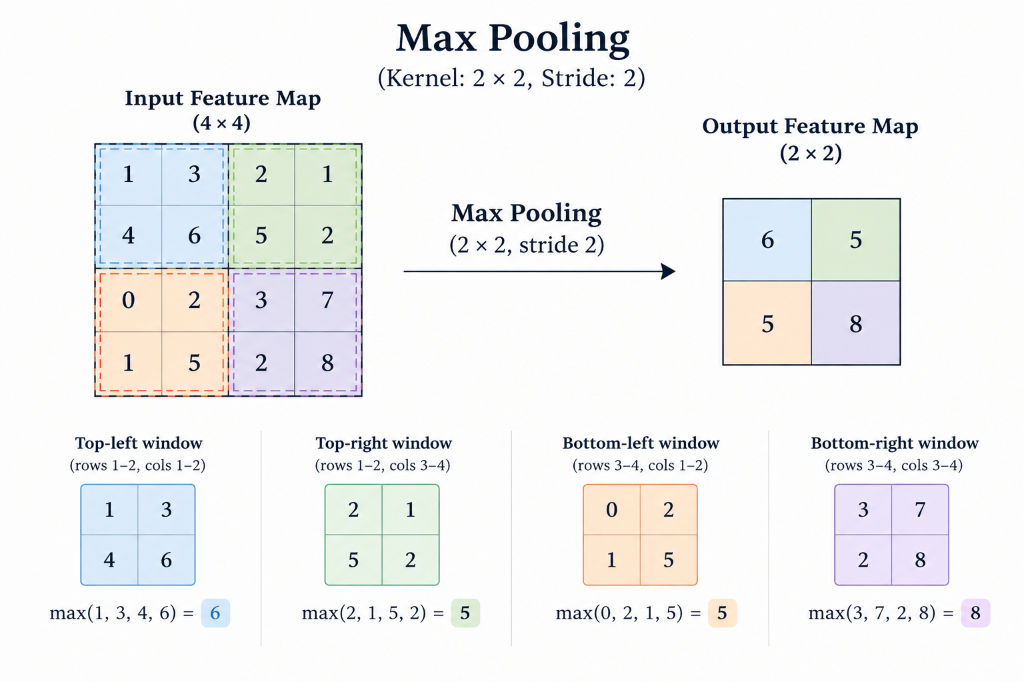
\includegraphics[width=0.95\textwidth]{figures/max_pooling.png}
\end{figure}
\begin{advbox}[Types of Pooling]
\begin{enumerate}[leftmargin=1.5em]
    \item \textbf{Max Pooling:} Selects the maximum value from each pooling window. It is the most commonly used pooling operation because it preserves the strongest features.
    \item \textbf{Average Pooling:} Computes the average value of each pooling window, producing a smoother feature map.
\end{enumerate}

\tcbline

\textbf{Note:} Pooling does not change the number of channels; it only reduces the height and width of the feature maps.

\textbf{Overlap Pooling (Stride = $2 \times 2$):} The windows touch each other but do not share any element (non-overlapping). If Stride = 1, the windows share many elements (overlapping).
\end{advbox}

\paragraph{Activation Function (Adding Non-Linearity)}

\begin{center}
\begin{minipage}{0.4\textwidth}
\centering
\textbf{Input Feature Map} \\[0.4em]
\begin{tabular}{|c|c|c|c|}
\hline
15 & 20 & 13 & -5 \\ \hline
250 & 15 & -4 & -3 \\ \hline
12 & 11 & 10 & 7 \\ \hline
-20 & 5 & -7 & 150 \\ \hline
\end{tabular}
\end{minipage}
\quad $\xrightarrow{\text{\textbf{ReLU}}}$ \quad
\begin{minipage}{0.4\textwidth}
\centering
\textbf{Activated Output} \\[0.4em]
\begin{tabular}{|c|c|c|c|}
\hline
15 & 20 & 13 & 0 \\ \hline
250 & 15 & 0 & 0 \\ \hline
12 & 11 & 10 & 7 \\ \hline
0 & 5 & 0 & 150 \\ \hline
\end{tabular}
\end{minipage}
\end{center}

\section{CNN Step-by-Step Pipeline}

\begin{propertybox}[Step-by-Step CNN Execution Flow]
\textbf{Input:} $28 \times 28 \times 3$
\begin{itemize}
    \item \textbf{Conv Layer 1:} 8 Kernels ($3 \times 3 \times 3$). Each kernel scans across all 3 channels simultaneously, summing them into one value per position $\to$ 8 Kernels = 8 output feature maps. \quad $\mathbf{\to \text{Output: } 26 \times 26 \times 8}$
    \item \textbf{Activation (ReLU):} Applied element-wise to all 8 feature maps.
    \item \textbf{Pooling (Max Pool $2 \times 2$):} $26 \times 26 \times 8 \to 13 \times 13 \times 8$
    \item \textbf{Conv Layer 2:} 16 Kernels ($3 \times 3 \times 8$) $\mathbf{\to \text{Output: } 11 \times 11 \times 16}$
    \item \textbf{Repeat Conv + Pool block}
    \item \textbf{Flatten $\to$ Linear (MLP) $\to$ Final Classification}
\end{itemize}
\end{propertybox}

\section{Backpropagation \& Parameter Gradients in CNNs}

Unlike traditional image processing filters such as Sobel or Gaussian chosen manually, CNNs treat the values within each kernel as learnable parameters. Kernel weights are set to small random values. Through the training process, these weights are iteratively updated using Gradient Descent following the backpropagation rule:

\begin{equation}
w_{m,n}^{(t+1)} = w_{m,n}^{(t)} - \eta \frac{\partial L}{\partial w_{m,n}}
\end{equation}

\paragraph{Gradient w.r.t. Kernel $w$:}
\begin{equation}
\frac{\partial L}{\partial w_{m,n}} = \sum_{i,j} \frac{\partial L}{\partial Y_{i,j}} \cdot \frac{\partial Y_{i,j}}{\partial w_{m,n}}, \qquad \text{where } \frac{\partial Y_{i,j}}{\partial w_{m,n}} = X_{i+m, j+n}
\end{equation}

\begin{equation}
\boxed{\frac{\partial L}{\partial w_{m,n}} = \sum_{i,j} dY_{i,j} \cdot X_{i+m, j+n}}
\end{equation}

\paragraph{Gradient w.r.t. Bias $b$:}
\begin{equation}
\frac{\partial L}{\partial b} = \sum_{i,j} dY_{i,j}
\end{equation}

\paragraph{Gradient w.r.t. Input $X$:}
\begin{equation}
\frac{\partial L}{\partial X_{p,q}} = \sum_{m,n} dY_{p-m, q-n} \cdot w_{m,n}
\end{equation}

\begin{center}
\textbf{Forward:} $X \xrightarrow{\quad \text{Conv} \quad} Y \qquad \mathbf{\vert} \qquad \textbf{Backward:} dY \xrightarrow{\quad dW, dX \quad} dX$
\end{center}

\section{Batch Normalization}

\begin{itemize}
    \item \textbf{Problem:} Feature scaling was applied only once, to the raw input $x$. But every hidden layer's output $z^{(k)}$ is also a feature vector whose scale drifts during training, causing the same slow-convergence problem as before.
    \item \textbf{Solution:} Standardize the output of every hidden layer at every training step — not just the input once.
\end{itemize}

\subsection{The Memory Problem \& Channel-Wise Solution}

Naively, Batch Normalization needs one $\mu$ (mean), $\sigma$ (standard deviation), $\gamma$, $\beta$ per pixel position. For a $150 \times 150 \times 64$ feature map, that requires:
\begin{equation}
4 \times 150 \times 150 \times 64 = 5.76\text{M parameters for one Batch Normalization layer}
\end{equation}

\textbf{Solution:} Share one scalar per channel instead of per pixel position. Make it $1 \times 1 \times 64$ instead of $150 \times 150 \times 64$. All spatial positions in a channel $R$ reuse the same $\gamma, \beta, \mu, \sigma$, reducing the count to:
\begin{equation}
4 \times 64 = \boxed{256 \text{ parameters}}
\end{equation}
\subsection{Keras Implementation}

\begin{verbatim}
model = models.Sequential()
model.add(layers.Conv2D(10, (5, 5), input_shape=(28, 28, 1)))
model.add(layers.BatchNormalization())
model.add(layers.Activation('relu'))
model.add(layers.MaxPooling2D((2, 2)))

model.add(layers.Conv2D(20, (5, 5)))
model.add(layers.BatchNormalization())
model.add(layers.Activation('relu'))
model.add(layers.MaxPooling2D((2, 2)))

model.add(layers.Flatten())
model.add(layers.Dense(10, activation='softmax'))
\end{verbatim}

\begin{table}[htbp]
\centering
\caption{Parameter Count Before and After Adding Batch Normalization}
\label{tab}
\begin{tabular}{lcc}
\toprule
\textbf{Layer} & \textbf{Without BN} & \textbf{With BN} \\
\midrule
Conv2D\_1 & 260 & 260 \\
Batch Normalization\_1 & -- & 40 \\
Conv2D\_2 & 5,020 & 5,020 \\
Batch Normalization\_2 & -- & 80 \\
Dense & 3,210 & 3,210 \\
\midrule
\textbf{Total Parameters} & \textbf{8,490} & \textbf{8,610} \\
\textbf{Additional Parameters} & -- & \textbf{120} \\
\bottomrule
\end{tabular}
\end{table}

The version with BN converges roughly $10\times$ faster, reaching $\sim 98\%$ accuracy in 3 epochs instead of $\sim 30$. The extra parameters ($0.2\text{ MB}$ difference, negligible) buy a massive gain in convergence speed and training stability.

\section{Common CNN Architectures}

\subsection{LeNet-5 (1998)}

LeNet-5, proposed by Yann LeCun, Léon Bottou, Yoshua Bengio, and Patrick Haffner in 1998, is one of the earliest and most influential Convolutional Neural Networks (CNNs). It was designed for handwritten digit recognition and achieved remarkable performance on the MNIST dataset, demonstrating the effectiveness of convolutional neural networks for image classification.

The architecture consists of a sequence of convolutional, subsampling (average pooling), and fully connected layers:

\begin{itemize}
    \item \textbf{Input Layer:} A grayscale image of size $32 \times 32$.
    
    \item \textbf{Convolution Layers:} Convolution operations using $5 \times 5$ kernels extract local features such as edges and simple patterns. The first convolution layer produces 6 feature maps, while the second produces 16 feature maps.

    \item \textbf{Subsampling Layers:} Average pooling with a $2 \times 2$ window reduces the spatial dimensions of the feature maps, decreases computational cost, and provides a degree of translation invariance.

    \item \textbf{Fully Connected Layers:} The extracted features are flattened and passed through fully connected layers that combine the learned representations.

    \item \textbf{Output Layer:} A final fully connected layer produces probabilities for the ten digit classes (0--9).
\end{itemize}

LeNet-5 introduced several fundamental concepts that became standard in modern deep learning, including local receptive fields, shared convolutional weights, pooling operations, and end-to-end learning through backpropagation. Although relatively small compared with modern CNNs, it established the foundation for many successful convolutional network architectures developed in later years.
\begin{figure}[H]
\centering
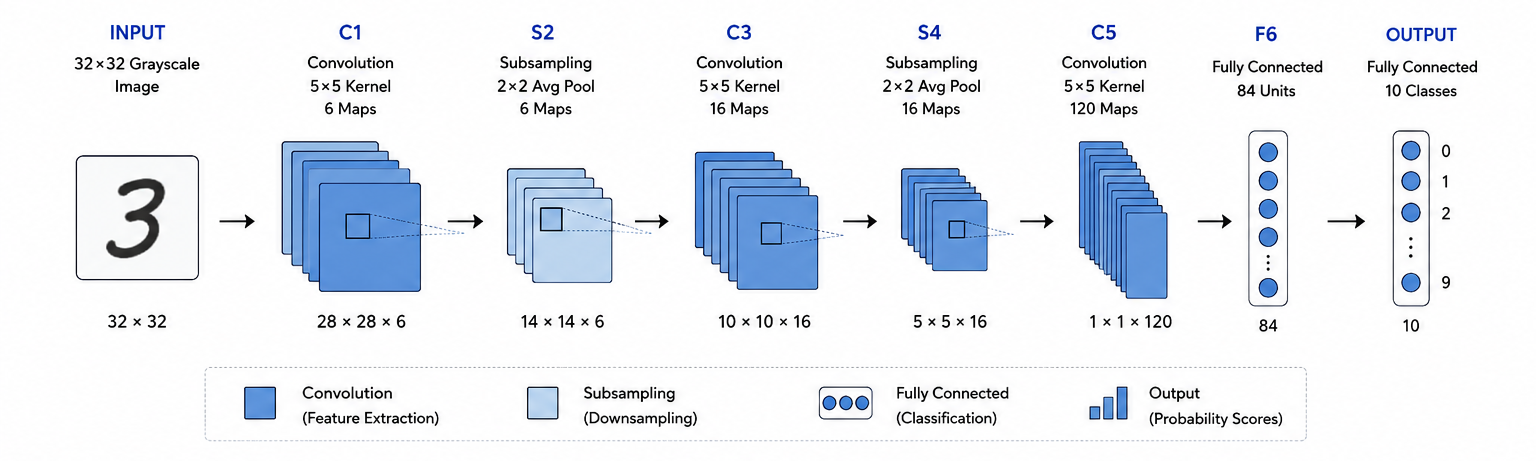
\includegraphics[width=0.95\textwidth]{figures/lenet1.png}
\end{figure}
\begin{figure}[H]
\centering
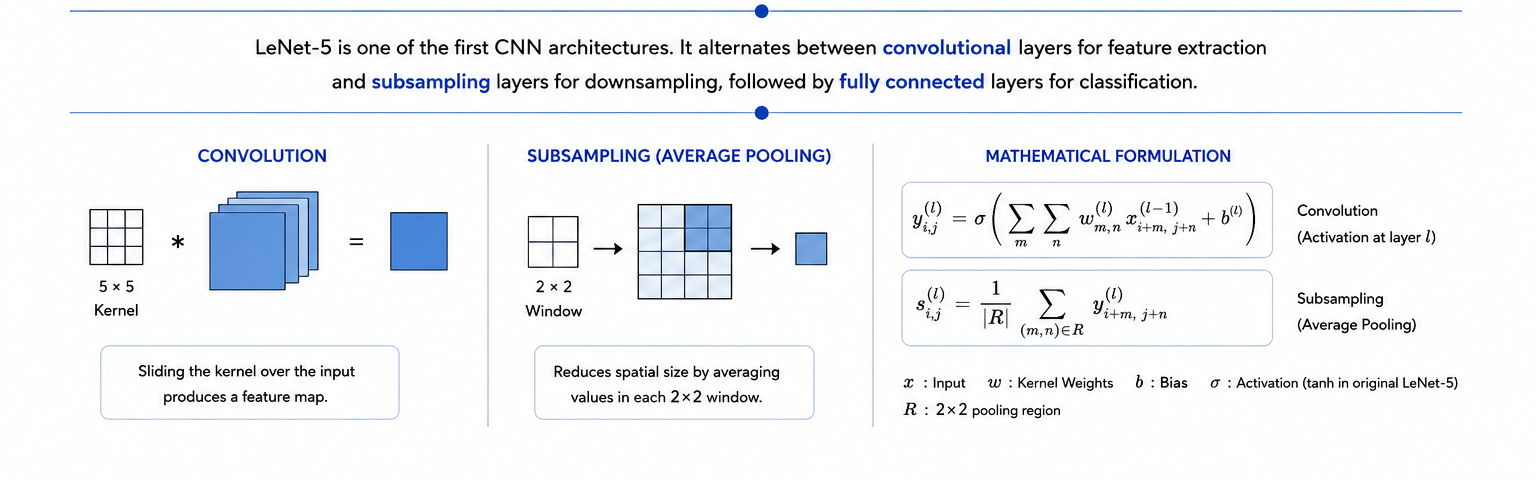
\includegraphics[width=0.95\textwidth]{figures/lenet2.png}
\end{figure}
\subsection{AlexNet (2012)}
5 Conv layers, 3 FC layers, 60M parameters. Key innovations:
\begin{enumerate}
    \item \textbf{ReLU instead of Sigmoid / Tanh:} Avoids the vanishing gradient problem.
    \item \textbf{Dropout in FC layers:} Acts as a regularizer to fight overfitting.
    \item \textbf{GPU Training:} Trained 1.2M images on GPUs instead of CPUs.
    \item \textbf{Large Stride and Kernels early ($11 \times 11$, Stride 4):} Aggressively downsamples big $224 \times 224$ inputs quickly, followed by smaller kernels ($5 \times 5, 3 \times 3$) deeper in.
\end{enumerate}
\begin{figure}[H]
\centering
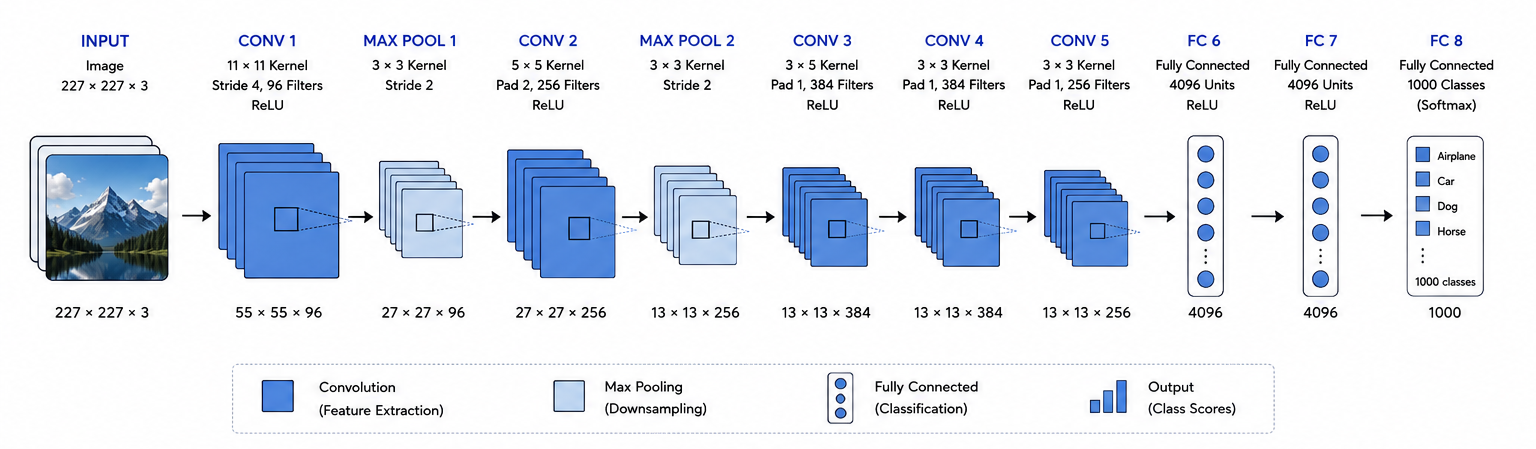
\includegraphics[width=0.95\textwidth]{figures/alexnet1.png}
\end{figure}
\begin{figure}[H]
\centering
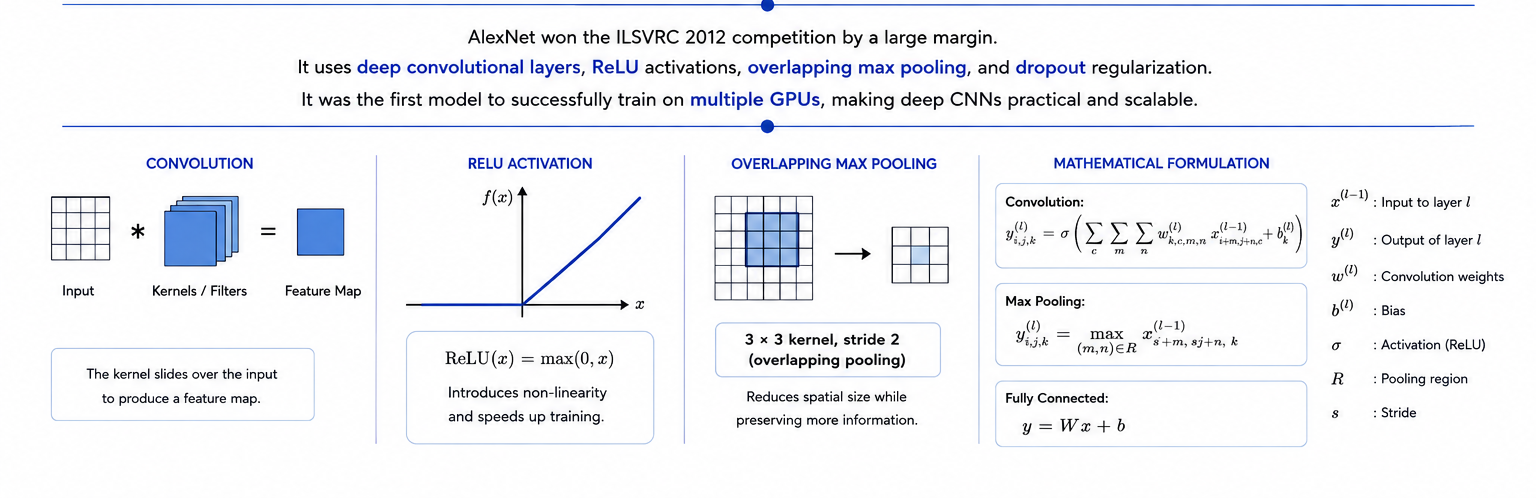
\includegraphics[width=0.95\textwidth]{figures/alexnet2.png}
\end{figure}
\begin{propertybox}[Historical Significance]
This is the paper that revived neural networks after the ``neural networks are dead'' period — winning ImageNet 2012 by a huge margin over traditional SIFT/HOG-based methods.
\end{propertybox}

\begin{center}
\begin{tikzpicture}[scale=0.85]
  \draw[-{Latex}, warmgray, line width=1pt] (0,0) -- (12,0) node[right, font=\sffamily\scriptsize] {Year};
  
  \foreach \x/\year/\label in {0.5/1943/First NN, 2.0/1958/Perceptron, 4.2/1986/RNN, 5.8/1997/LSTM, 7.0/1998/LeNet, 10.5/2012/AlexNet} {
    \draw[primaryblue, fill=white, line width=1pt] (\x,0) circle (3pt);
    \node[above=4pt, font=\sffamily\tiny\bfseries, color=primaryblue] at (\x,0) {\label};
    \node[below=4pt, font=\sffamily\tiny, color=warmgray] at (\x,0) {\year};
  }
  
  \draw[accentred, dashed, line width=0.8pt] (7.1,-0.6) -- (10.4,-0.6);
  \node[below=8pt, font=\sffamily\tiny, color=accentred, align=center] at (8.75,-0.5) {``NN were considered Dead\\by most ML researchers''};
\end{tikzpicture}
\end{center}

\subsection{VGG-16 (2014)}

VGG-16, proposed by Karen Simonyan and Andrew Zisserman in 2014, is a deep Convolutional Neural Network (CNN) known for its simple and uniform architecture. It uses only $3 \times 3$ convolution filters and consists of 13 convolutional layers followed by 3 fully connected layers (16 weight layers in total), with approximately 138 million trainable parameters. Despite its high computational cost, VGG-16 achieved excellent performance on ImageNet and became a widely used backbone for image classification, object detection, semantic segmentation, and transfer learning.

\begin{itemize}
    \item \textbf{Uniformity and depth via small kernels:} Instead of AlexNet's mix of large and small kernels, VGG uses only $3 \times 3$ convolutions stacked repeatedly before each pooling step, providing fewer parameters and extra non-linearity.
    \item \textbf{Fine-Tuning pattern still used today:} Freeze early conv blocks (1 to 4, generic features), fine-tune only the last conv block + custom FC head for a new task.
\end{itemize}
\begin{figure}[H]
\centering
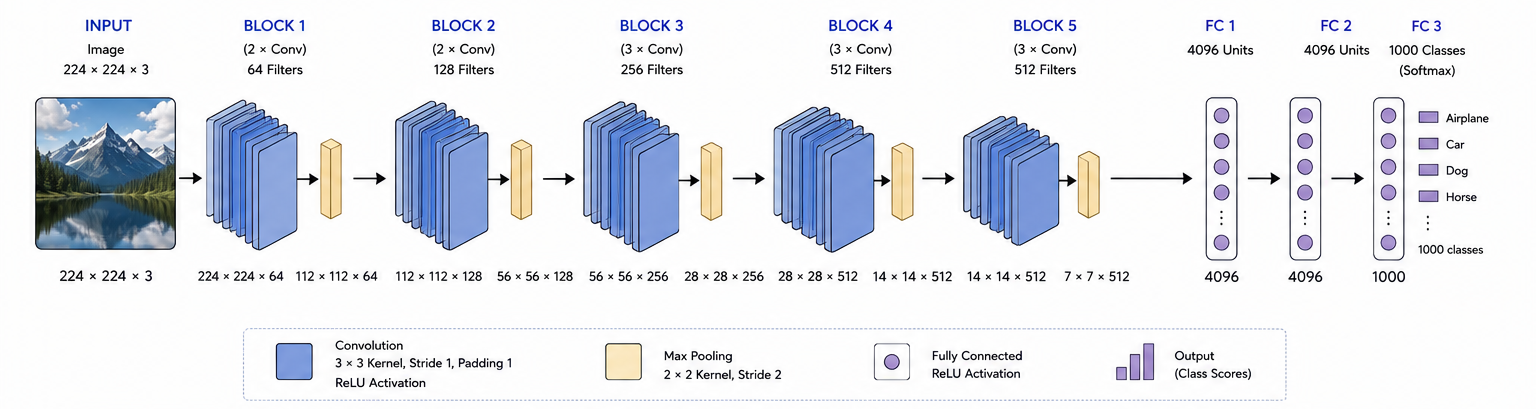
\includegraphics[width=0.95\textwidth]{figures/vgg1.png}
\end{figure}
\begin{figure}[H]
\centering
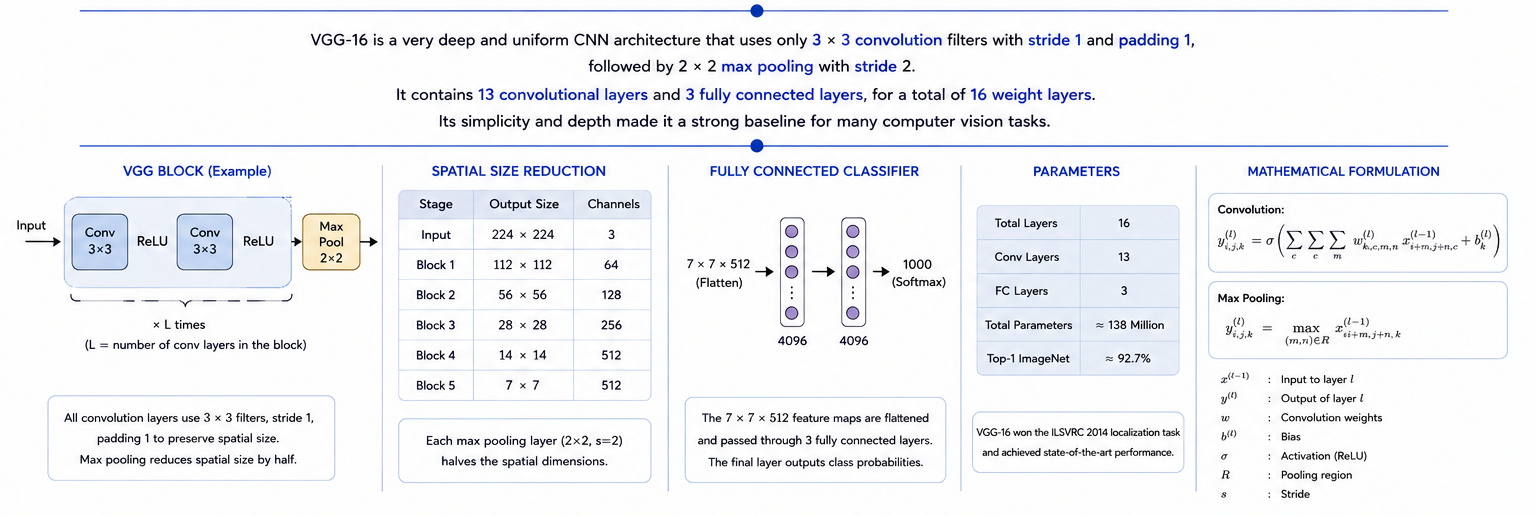
\includegraphics[width=0.95\textwidth]{figures/vgg2.png}
\end{figure}
\paragraph{Why Not Just Keep Stacking VGG-Style?}
Pushing plain sequential architectures past $\sim 20$ layers made both training and test error worse — not due to overfitting, but due to \textbf{vanishing gradients}.

\subsection{GoogLeNet / Inception (2014 / 2015)}
21 Conv layers + 1 FC layer, 5M parameters.
\begin{enumerate}
    \item \textbf{Inception Module:} Runs $1 \times 1$, $3 \times 3$, $5 \times 5$ convolutions and $3 \times 3$ max-pooling in parallel, then concatenates their outputs. The $1 \times 1$ convolution reduces dimensions before the $3 \times 3$ and $5 \times 5$ branches, keeping the model efficient (5M params vs VGG-16's 138M).
    \item \textbf{Auxiliary Outputs:} Extra Softmax classifiers added to intermediate layers during training only to provide direct gradients to earlier layers. Removed during inference.
    \item \textbf{Global Average Pooling instead of Flatten:} Replaces large Flatten + FC layers with Global Average Pooling, reducing feature maps to $1 \times 1 \times 1024$ before the final FC (1000) layer.
\end{enumerate}

\subsection{ResNet (2015)}
Up to 151 Conv layers + 1 FC layer. Introduces \textbf{Skip (residual) connections}:
\begin{equation}
y = F(x) + x
\end{equation}

Instead of learning the full mapping, the network learns the residual $F(x)$ and adds the original input $x$.
\begin{figure}[H]
\centering
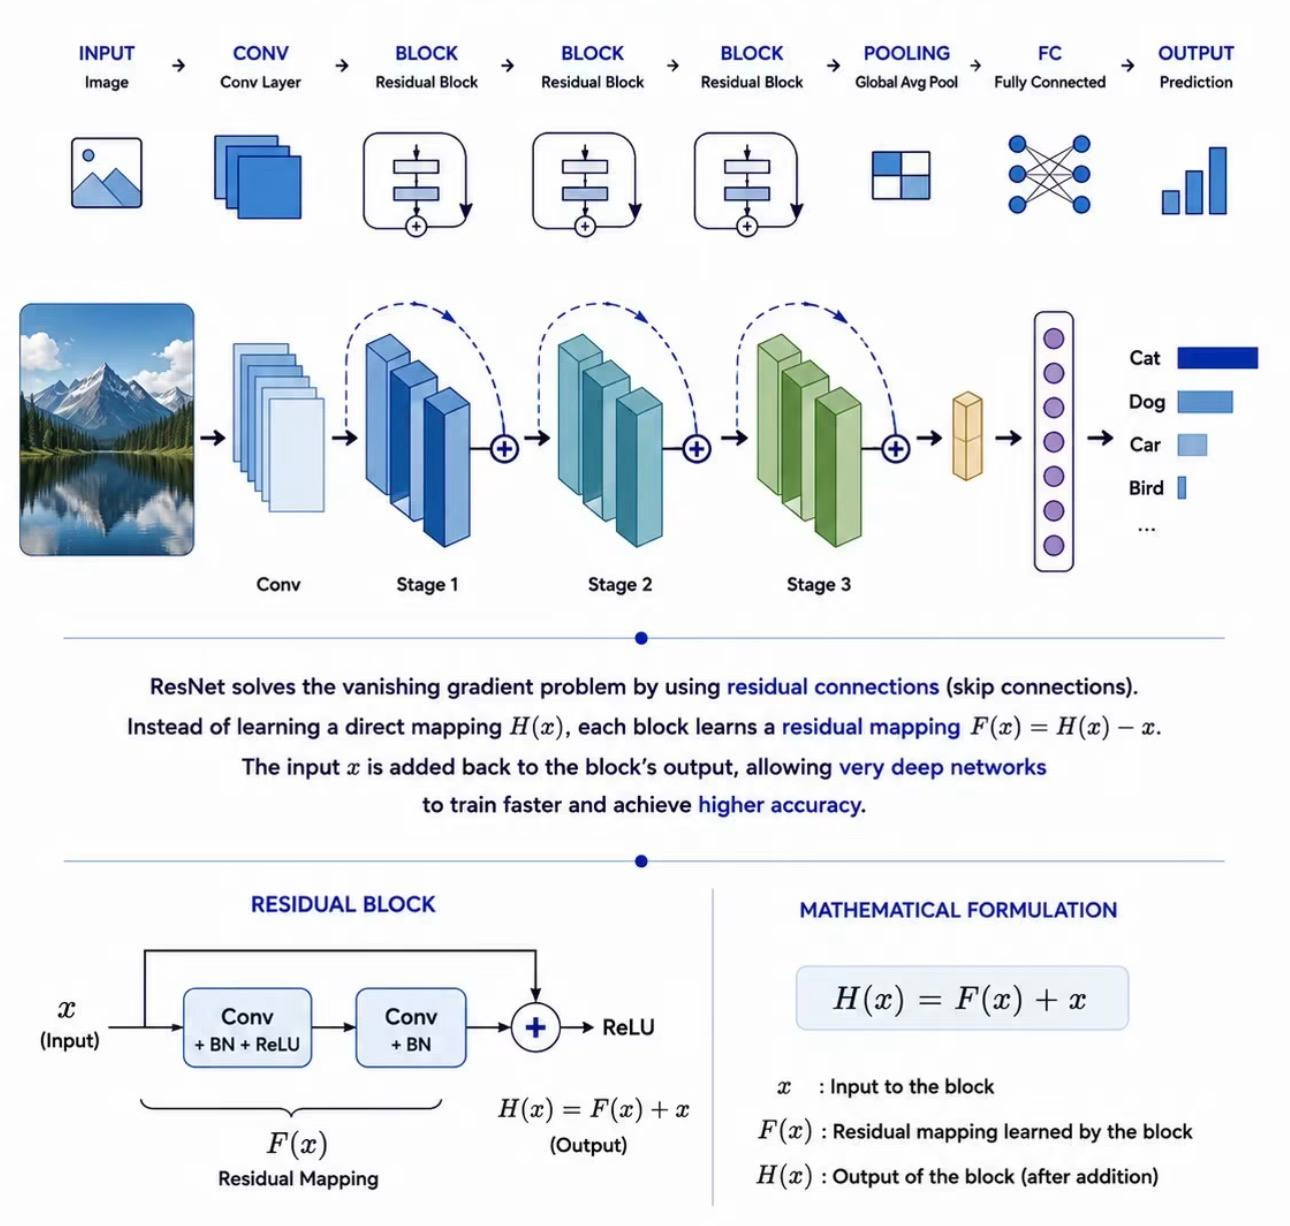
\includegraphics[width=0.95\textwidth]{figures/resnet.jpg}
\end{figure}
\paragraph{Why It Solved Vanishing Gradients:}
The identity connection $+x$ creates a direct gradient path:
\begin{equation}
\frac{\partial y}{\partial x} = \frac{\partial F(x)}{\partial x} + I
\end{equation}

The $I$ (identity) term acts as a gradient ``highway'', allowing gradients to flow even if $\frac{\partial F(x)}{\partial x}$ becomes very small. ResNet successfully trained 152 layers ($\sim 7\times$ deeper than VGG16), proving that deeper performance drops were optimization issues rather than limits of Deep Learning.

\subsection{U-Net (2015)}

U-Net is a convolutional neural network introduced by Olaf Ronneberger, Philipp Fischer, and Thomas Brox in 2015 for biomedical image segmentation. It follows an encoder--decoder architecture with symmetric skip connections, allowing the network to capture both high-level semantic information and fine spatial details.

The architecture consists of four main components:

\begin{itemize}
    \item \textbf{Encoder (Contracting Path):} Repeated applications of two $3\times3$ convolutions followed by ReLU activation and a $2\times2$ max pooling operation. The spatial resolution decreases while the number of feature channels increases.

    \item \textbf{Bottleneck:} The deepest part of the network, where feature maps contain the highest-level semantic information before reconstruction begins.

    \item \textbf{Decoder (Expanding Path):} Each stage performs upsampling using transposed convolution (or up-convolution), concatenates the corresponding encoder feature maps through skip connections, and applies two $3\times3$ convolutions with ReLU activation.

    \item \textbf{Output Layer:} A final $1\times1$ convolution maps the extracted features to the desired number of segmentation classes, producing a pixel-wise prediction.
\end{itemize}

The skip connections preserve high-resolution information lost during downsampling, enabling accurate localization while maintaining rich contextual information. This design makes U-Net highly effective for semantic segmentation tasks, especially when training data is limited.
\begin{figure}[H]
\centering
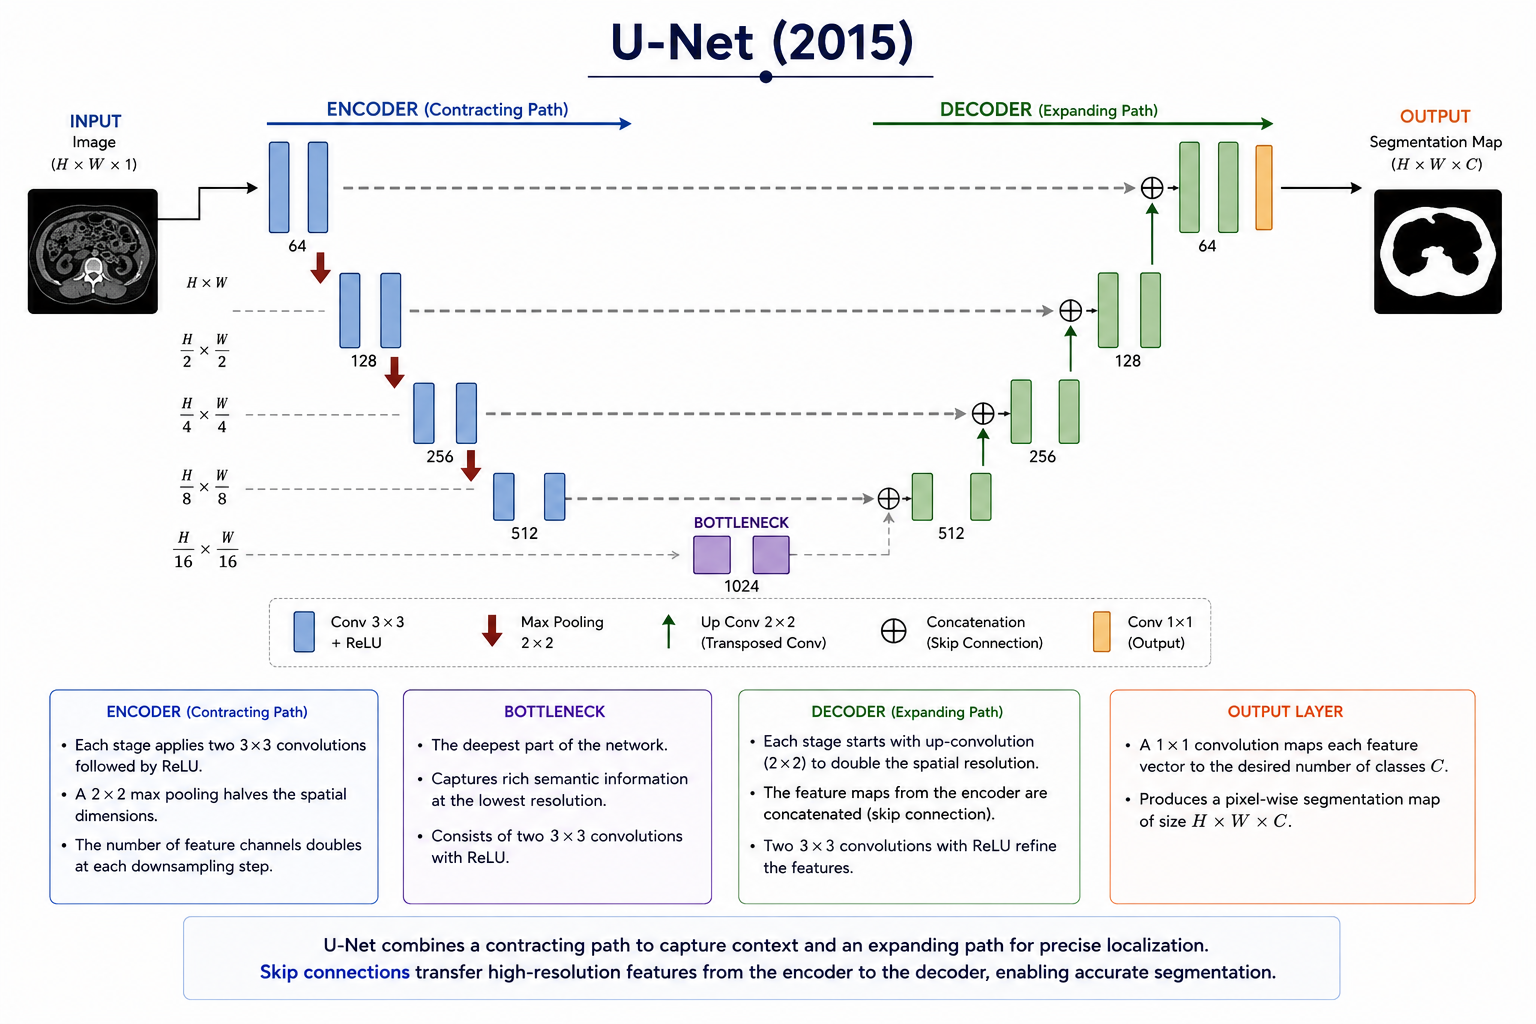
\includegraphics[width=0.95\textwidth]{figures/unet.png}
\end{figure}
\subsection{MobileNet (2017)}
Key Innovation ($\sim 4\text{M}$ parameters), designed specifically for mobile and edge devices.
\begin{enumerate}
    \item \textbf{Depthwise Separable Convolution:} Splits standard convolution into two steps:
    \begin{itemize}
        \item \textbf{Depthwise Convolution:} Applies one filter to each input channel separately.
        \item \textbf{Pointwise ($1 \times 1$) Convolution:} Combines information across channels.
    \end{itemize}
    \item \textbf{Global Average Pooling instead of Flatten:} Significantly reduces parameter count.
\end{enumerate}

MobileNet addressed the edge deployment problem by making CNNs small and efficient enough to run directly on smartphones and edge devices, reducing cloud reliance and improving latency, privacy, and memory efficiency.
 \begin{figure}[H]
\centering
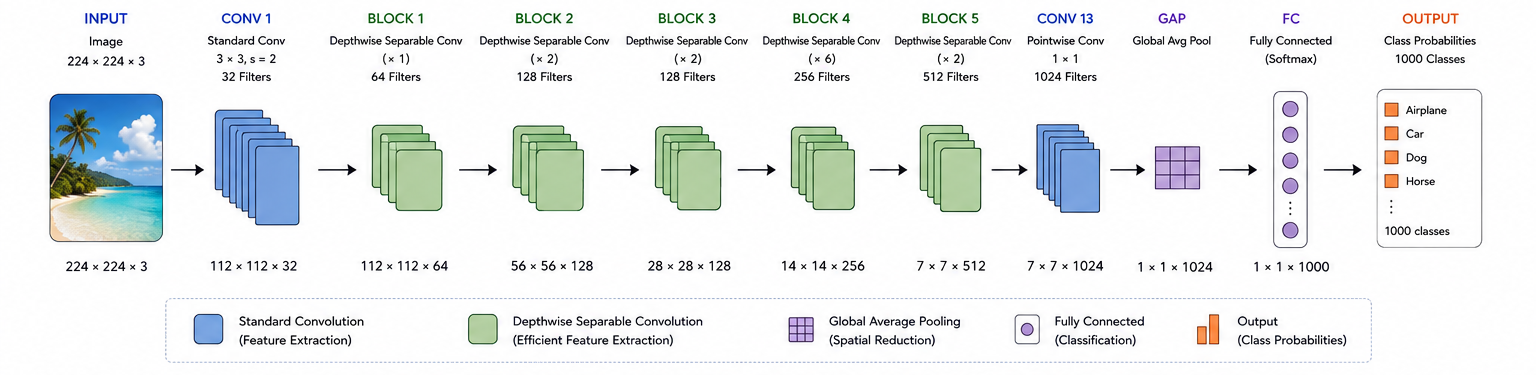
\includegraphics[width=0.95\textwidth]{figures/mobilenet1.png}
\end{figure}
 \begin{figure}[H]
\centering
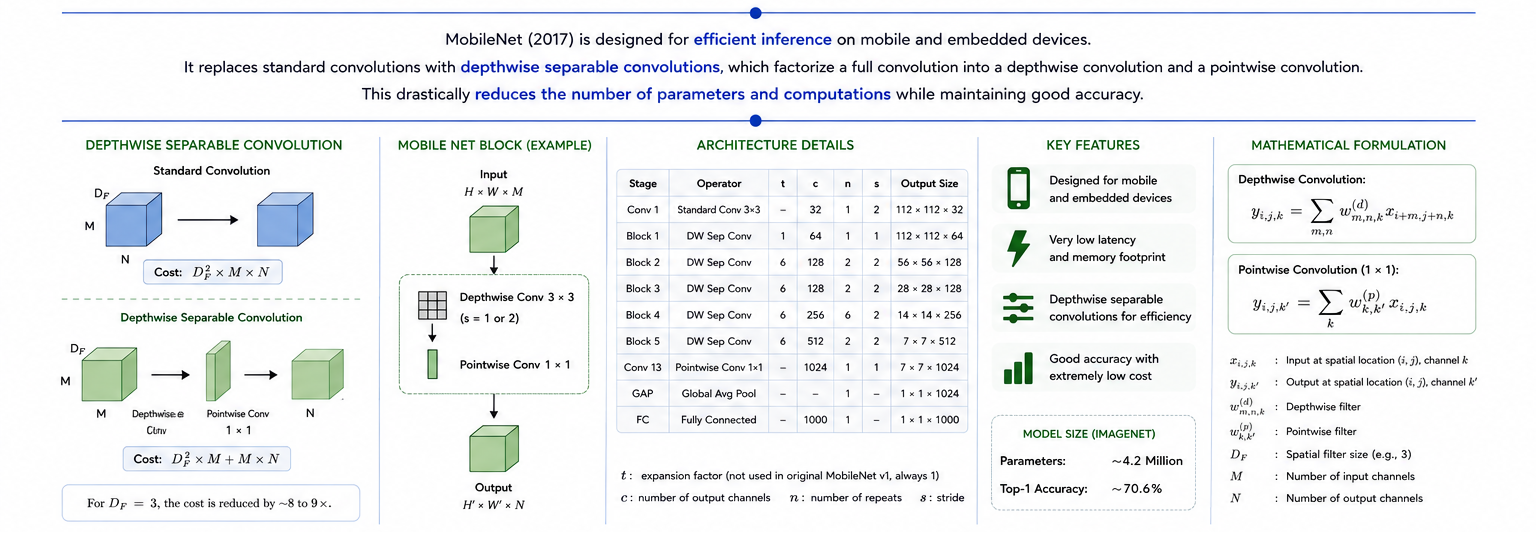
\includegraphics[width=0.95\textwidth]{figures/mobilenet2.png}
\end{figure}
